\section{Polytopes and combinatorial manifolds}

We will use two types of classical combinatorial structures: \emph{abstract polytopes} and \emph{combinatorial manifolds}. The latter is a subtype of the former. Abstract polytopes (or just ``polytopes'' in this note) encompass polygons, polyhedra, and higher-dimensional versions. They exclude certain undesirable shapes such as two triangles that meet at one vertex. But they aren't necessarily simplicial either:


\begin{verbatim}

Meeting with Mathieu 11/27:
an angle is: a path in S1 from base, which is equiv to a path in AutS1 from the identity to another automorphism. (automorphism is primary: aut of tangent circle)
viewed as automorphisms we can compose them.
viewed as paths, multiply path 2 by the element at the endpoint of path 1.


Curvature maps a loop in the base to a path in automorphisms of the tangent circle at the base.

A vector field + a trivialization ("fiducial v.f.") maps a loop in the base to the tangent circle at the basepoint. We can take the index/degree of this.

given a loop L:v=v, v.f. F, take F(L):tr_L(F(v))=F(v) ("apd", dependent action on paths).

type family f:A->U, \prod_{a:A}fa is the type of dependent functions
let X:\prod_{a:A}fa
we can apply X to a path p:a=_A b
X(p) is a path over p
X(p):tr_p(X(a))=X(b)
X(a), X(b) are terms of different types

covariant derivative of F along itself: lift F to F' horizontal on TP (P->M), take [F', F']

tangent bundle TM->M w/ connection \omega
covariant derivative of F in the direction of X \nabla_X(F)(x). 
1. lift X and F to horizontal fields X', F' in TTM
2. compute [X', F'] to TTM
3. decompose [X', F'] = [X, F]' + \omega([X', F'])

Use this:
\nabla_X(F) = [X, F] + \omega(X)(F)
Now take X=F
\nabla_F(F) = [F, F] + \omega(F)(F) = \omega(F)(F)

Meeting with steve:
the ctors present the HIT, and the HIT is a type.
universe must be closed under inductive types.
polygons of different cardinality will tangle with transport.


Minimal HITs:

def S1:
base: S1
loop: base=base

def S2:
N: S2
surf: refl_N = refl_N

def torus:
b:torus
p,q:b=b
donut:p.q=q.p


the map R (realization) R(S2):U lossy map

R(C_4) has an equivalence to R(S1)
perhaps this is R(the map C_4->S1, the strict one)
C_4->S1 is a strict map
S1->C_4 is non-strict, uses generated data, uses data from R(C_4)

def OO:
6 vertices
12 edges
8 faces

f:S2->OO 
T:OO->EM(Z,1)

def OO_w:
5 vertices
8 edges
5 faces: four bottom triangles, and a square refl_b=loop "brgob"

g:S2->OO_w

compose f and g^{-1} to give OO equiv OO_w

Tof(base) is (C_4, is_equiv_s1)
inside this is a twice rotation around C_4 and a homotopy to id(C_4)

"strict morphism of HITs": ctors to ctors

Imagine only having X:U, or X:*-> U

Claim: we cannot see the one-notch "90 degree" rotation of C_4 at the level of types.

-- Connections --
Type X w/ 1-skel X_1
HIT gives skeletal filtration
functions naturally given as per-skeleton steps
there are constraints/obstructions:
obstruction to extend map T from vertices a, b to path e:a=b is that T(a) and T(b) are in same connected component
say 2-cell F contracts a loop L: F:L=refl_v some vertex v
we have a choice of v for each face F
then T(F) must be in same component as refl_v (refl_v:\pi_1 X with basepoint v)
T(F) is merely refl, and holonomy is merely refl, and connection on this face F is merely flat
curvature is a function from 2-cells to \pi_1(X,v)
T(v):U
T(L):T(v)=T(v)

T(F):refl_{T(v)}=T(L)
the class ||T(L)||:\pi_1(U,T(v)) is an obstruction to having T(F), to extending T to F

The hierarchy of maps extending to higher skeletons, which we call connections of dimension 1, 2, etc.
This works for ANY HIT.
The combinatorial manifold structure is just one special case that gives me a specific map T.
\end{verbatim}

\subsection{Polytopes}

\begin{mydef}
A \defemph{finite abstract polytope} \( \mathcal{P} \) of dimension \( n \) is a finite poset \( P \) equipped with 
\begin{itemize}
\item two elements \( p_{\mathrm{min}}, p_{\mathrm{max}}:P \)
\item a \emph{rank} function \( r:P\to \zz \)
\end{itemize}
and properties
\begin{itemize}
\item a proof that \( a\leq b\to r(a)\leq r(b) \)
\item a proof that \( p_{\mathrm{min}} \) is minimal: \( \pit{p:P}p\geq p_{\mathrm{min}} \)
\item a proof that \( p_{\mathrm{max}} \) is maximal: \( \pit{p:P}p\leq p_{\mathrm{max}} \)
\item a proof that \( r(p_{\mathrm{min}}) = -1 \) (so that non-minimal elements have rank at least 0)
\item a proof that \( r(p_{\mathrm{max}}) = n+1 \) (so that non-maximal elements have rank at most \( n \))
\item a proof that rank ``counts containment'': \( \pit{a,b:P}(a\leq b)\times (\mathsf{is\_empty}\sit{c:P}(a\leq c\leq b))\to b=a+1 \)
\item a proof of \emph{strong connectedness} (all intervals are connected via a chain of containment): \newline\( \pit{a,b:P\setminus\{p_{\mathrm{min}}, p_{\mathrm{max}}\}}\left(\sit{x:P}a\leq x\leq b\text{ is connected}\right) \)
\item a proof of the \emph{diamond condition} that between two elements that differ by two ranks lie exactly two elements: \( \pit{a,b:P}(r(b)-r(a)=2)\to \#(\sit{c:P}a\leq c\leq b)=4 \) (of which \( a \) and \( b \) are two).
\end{itemize}
\end{mydef}

The diamond condition captures that two edges meet at a vertex, two faces meet at one edge, and so on. See the Hasse diagram (a graph of the poset with rank represented on the \( y \)-axis) of a tetrahedron in Figure~\ref{fig:hasse_tetrahedron} and the square pyramid (which will arise later as an octahedron minus its south pole) in Figure~\ref{fig:hasse_pyramid}.

\begin{figure}[htbp]
\centering
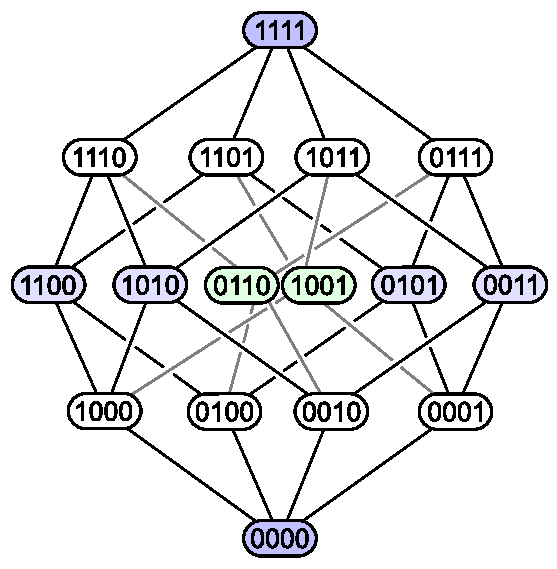
\includegraphics[width=200pt]{hasse_tetrahedron.pdf}
\caption{A finite abstract polytope representation of a tetrahedron, in the form of its ``Hasse diagram'' (from polytope.miraheze.org, public domain).}
\label{fig:hasse_tetrahedron}
\end{figure}

\begin{figure}[htbp]
\centering
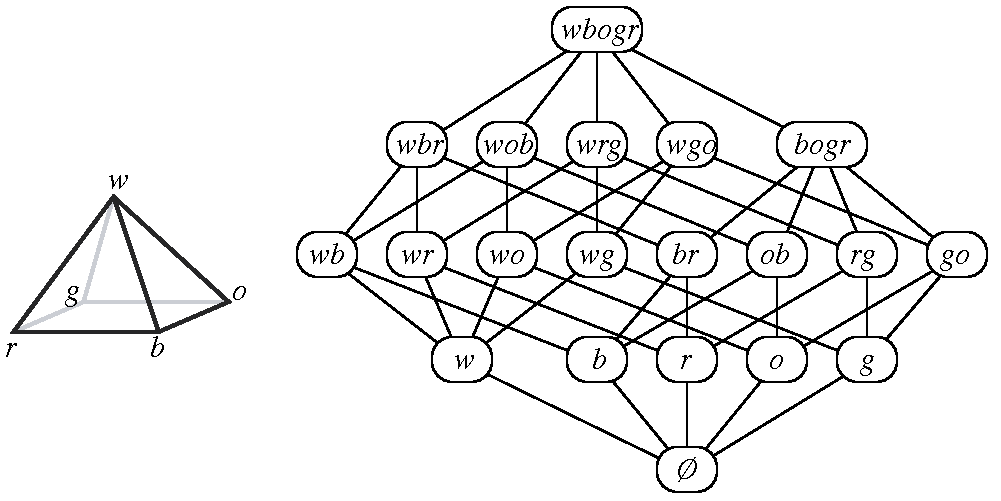
\includegraphics[width=350pt]{pyramid.pdf}
\caption{The Hasse diagram of a square pyramid (from wikimedia.org, public domain).}
\label{fig:hasse_pyramid}
\end{figure}

Next we will map abstract polytopes to higher inductive types. The poset structure will generate the paths, so the rank will correspond to the dimension. But as usual in a HIT we will need to make a choice of direction for each path constructor, which wasn't necessary in the polytope setting. We will restrict to dimension at most 2.

\begin{mydef}
A \defemph{higher inductive polytope (HIP) of dimension at most 2} \( \P \) for a polytope \( \mathcal{P} \) of dimension at most 2 is a type with constructor data given by
\begin{enumerate}
\item For each rank 0 element \( v \) a term \( V:\P \).
\item For each rank 1 element \( e \) and rank 1 pair \( v_1,v_2\leq e \) (cardinality 2 by the diamond condition) a path \( E:V_1=V_2 \).
\item For each rank 2 element \( f \) containing edges \( e_1,\ldots,e_n \) containing a cycle of vertex pairs \( \{\{v_{11},v_{12}\},\ldots,\{v_{n1},v_{n2}=v_{11}\}\} \) a 2-path \( F:E_1\cdot\ldots\cdot E_n=\refl_{v_{11}} \).
\end{enumerate}
\end{mydef}

\begin{mydef}
Given a HIT of dimension at most 2 we have the \defemph{skeleta} \( \P_0,\P_1,\P_2 \) where \( \P_i \) is the HIT generated by using the constructors up to dimension \( i \). The HIT also provides a chain of inclusions of skeleta \( \P_0\to\P_1\to\P_2 \).
\end{mydef}

If \( Z:\uni \) is a type then to define a map \( \P\to Z \) we start with a map \( \P\to Z \) and extend it to \( \P_1 \) and then \( \P_2 \). 

\subsection{Combinatorial manifolds}

We will adapt to higher inductive types in a straightforward manner the classical construction of \emph{combinatorial manifolds}. See for example the classic book by Kirby and Siebenmann\cite{kirby_siebenmann}. These are a subclass of simplicial complexes.

\begin{mydef}
An \defemph{abstract simplicial complex \( M \) of dimension \( n \)} consists of a set \( M_0 \) of vertices, and for each \( 0<k\leq n \) a set \( M_k \) of subsets of \( M_0 \) of cardinality \( k+1 \), such that any \( (j+1) \)-element subset of \( M_k \) is an element of \( M_j \). The elements of \( M_k \) are called \defemph{\( k \)-faces}. Denote by \( \simcomp \) the type of abstract simplicial complexes of dimension \( n \) (where the suffix \( \mathsf{Set} \) reminds us that this is a type of sets).
\end{mydef}

Note that we don't require all subsets of \( M_0 \) to be included -- that would make \( M \) an individual simplex. A simplicial complex is a family of simplices that are identified along various faces.

\begin{mydef}
In an abstract simplicial complex \( M \) of dimension \( n \), the \defemph{link} of a vertex \( v \) is the \( n-1 \)-face containing every face \( m\in M_{n-1} \) such that \( v\notin m \) and \( m\cup v \) is an \( n \)-face of \( M \).
\end{mydef}

The link is all the neighboring vertices of \( v \) and the codimension 1 faces joining those to each other. See for example Figure~\ref{fig:link}.

\begin{figure}[htbp]
\centering
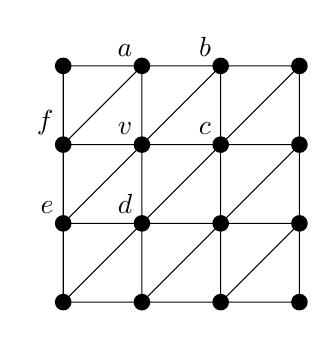
\begin{tikzpicture}
  \draw
    (0, 0) grid[step=1cm] (3, 3)
    (0, 2) -- (1, 3)
    (0, 1) -- (2, 3)
    (0, 0) -- (3, 3)
    (1, 0) -- (3, 2)
    (2, 0) -- (3, 1)
  ;
  \fill[radius=3pt]
    \foreach \x in {0, ..., 3} {
      \foreach \y in {0, ..., 3} {
        (\x, \y) circle[]
      }
    }
  ;
  \path[above left]
    \foreach \p/\v in {
      {1, 3}/a,
      {2, 3}/b,
      {0, 2}/f,
      {1, 2}/v,
      {2, 2}/c,
      {0, 1}/e,
      {1, 1}/d%
    } {
      (\p) node {$\v$}
    }
  ;
\end{tikzpicture}
\caption{The link of \( v \) in this complex consists of the vertices \( \{a,b,c,d,e,f\} \) and the edges \( \{ab,bc,cd,de,ef,fa\} \), forming a hexagon.}
\label{fig:link}
\end{figure}

\begin{mydef}
A \defemph{combinatorial manifold} (or \defemph{combinatorial triangulation}) of dimension \( n \) is a simplicial complex of dimension \( n \) such that the link of every vertex is a simplicial sphere of dimension \( n-1 \) (i.e. its geometric realization is homeomorphic to an \( n-1 \)-sphere). Denote by \( \combmfdset \) the type of combinatorial manifolds of dimension \( n \) (which the notation again reminds us are sets).
\end{mydef}

In a 2-dimensional combinatorial manifold the link is a polygon. See Figures~\ref{fig:sphere_triangulation}, \ref{fig:torus_wiki_triangulation}, and \ref{fig:genus3_wiki_triangulation} for some examples of 2-dimensional combinatorial manifolds of genus 0, 1, and 3.

A classical 1940 result of Whitehead, building on Cairn, states that every smooth manifold admits a combinatorial triangulation\cite{whitehead_triangulation}. So it appears reasonably well motivated to study this class of objects.

\begin{figure}[htbp]
\centering
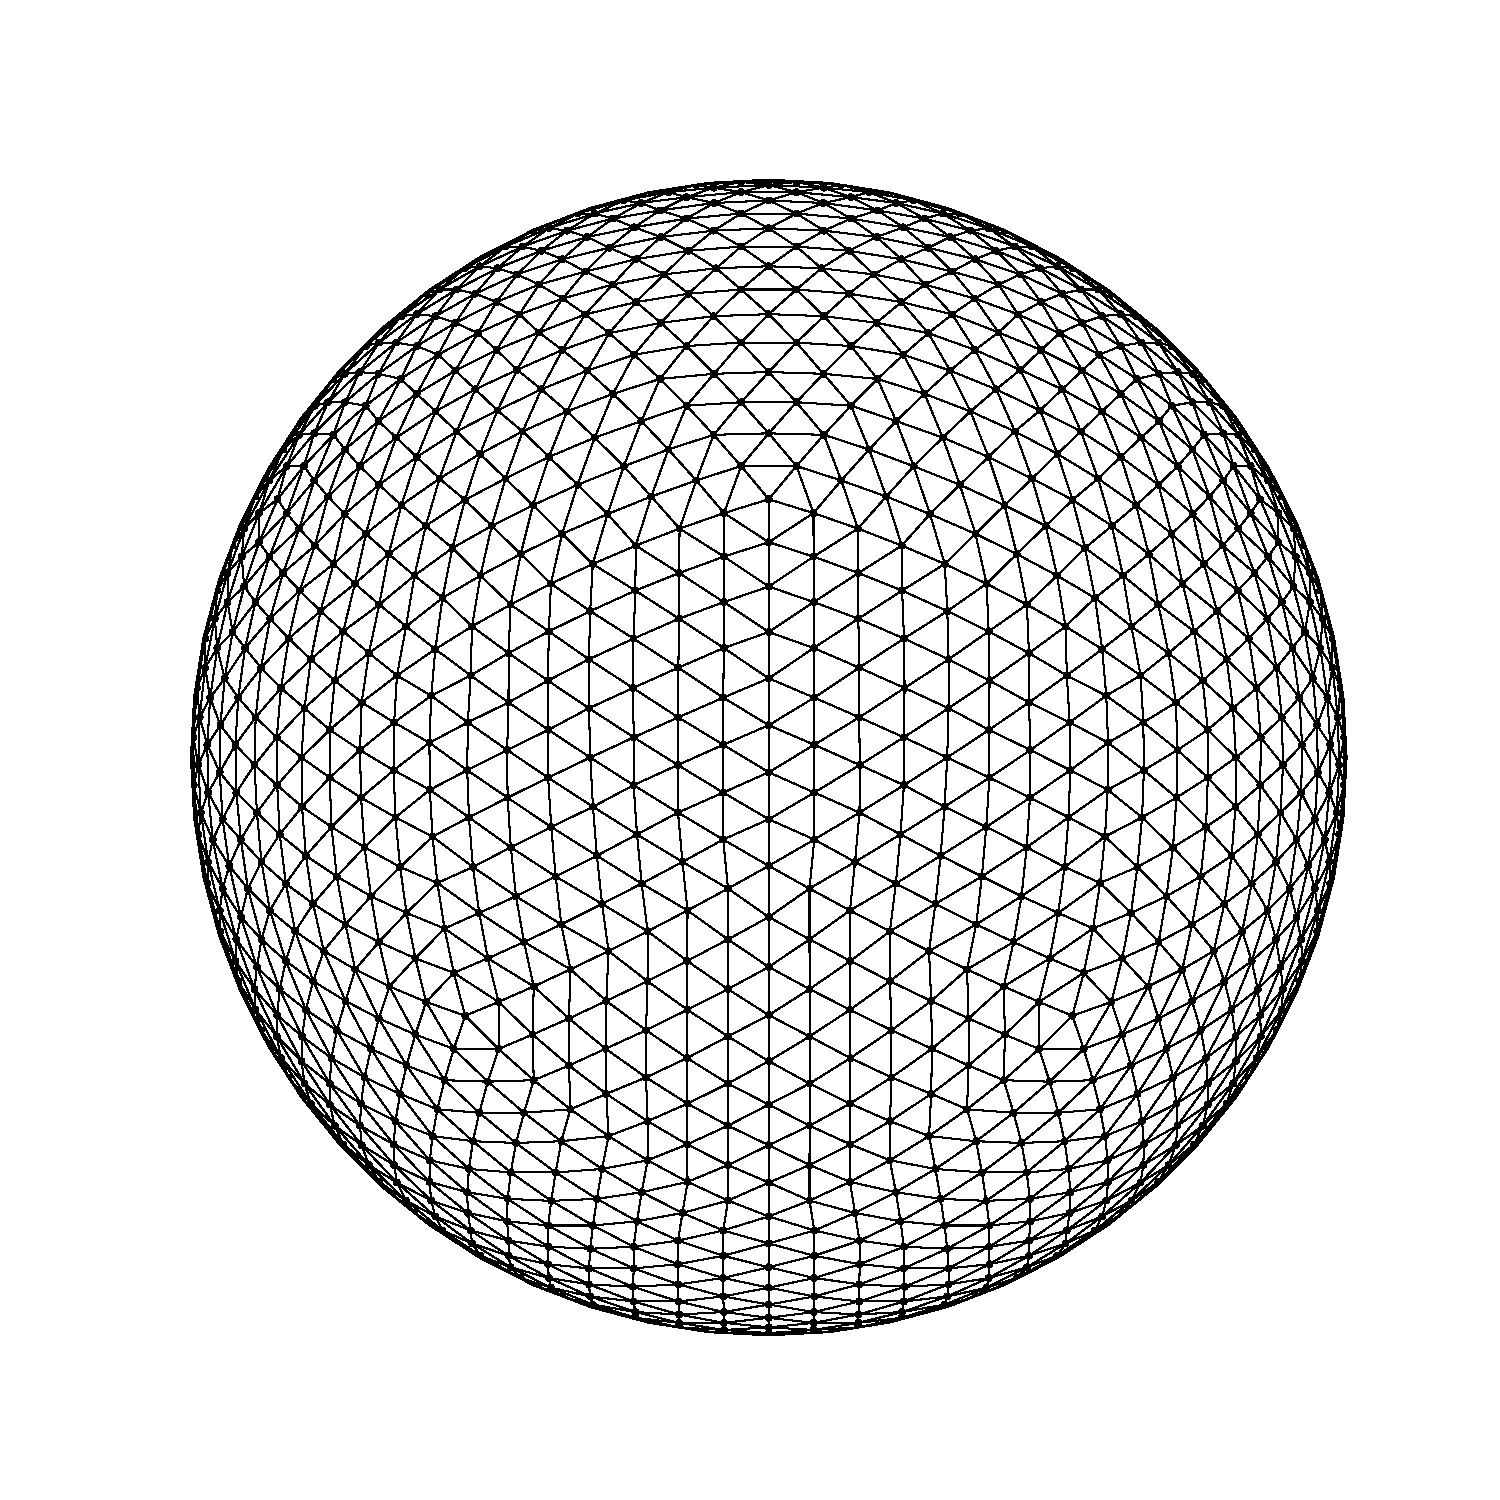
\includegraphics[width=200pt]{triangulated_sphere.pdf}
\caption{A combinatorial triangulation of a sphere, created with the tool \texttt{stripy}.}
\label{fig:sphere_triangulation}
\end{figure}

\begin{figure}[htbp]
\centering
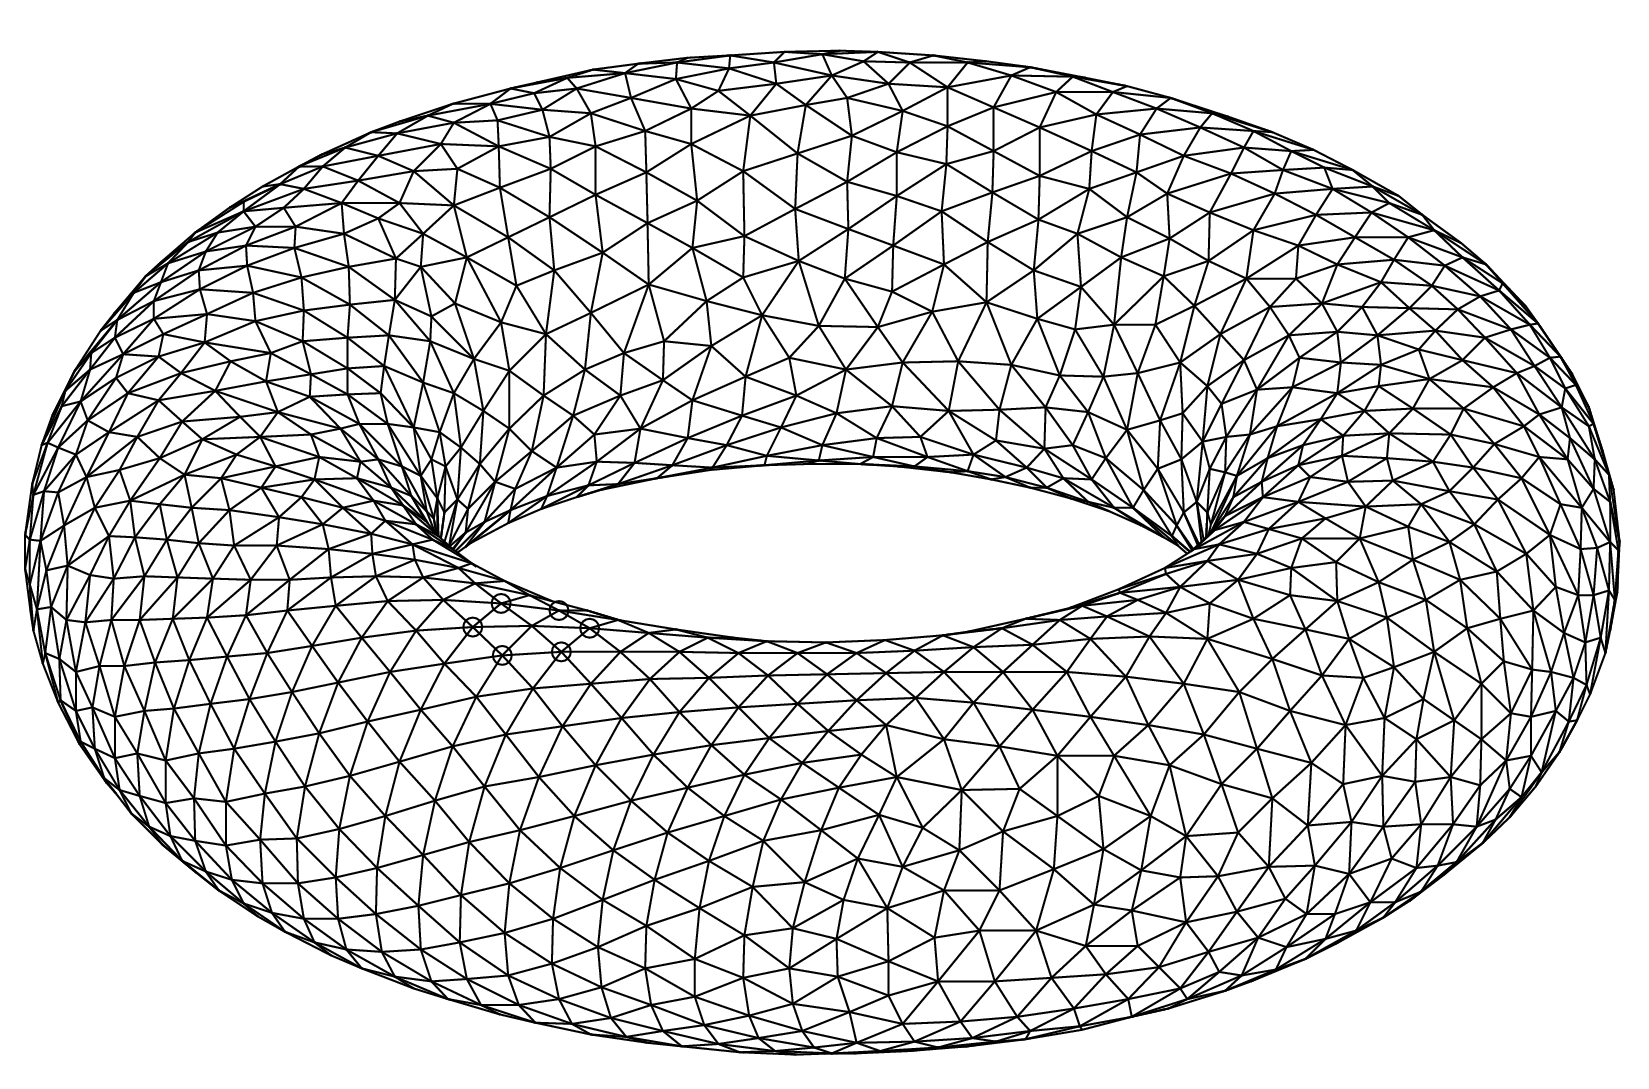
\includegraphics[width=200pt]{Torus-triang.png}
\caption{A torus with an interesting triangulation, from Wikipedia. The links have various vertex counts from 5-7. Clearly a constant value of 6 would also work. (\href{https://commons.wikimedia.org/w/index.php?curid=30856793}{By Ag2gaeh} - Own work, CC BY-SA 3.0.)}
\label{fig:torus_wiki_triangulation}
\end{figure}

\begin{figure}[htbp]
\centering
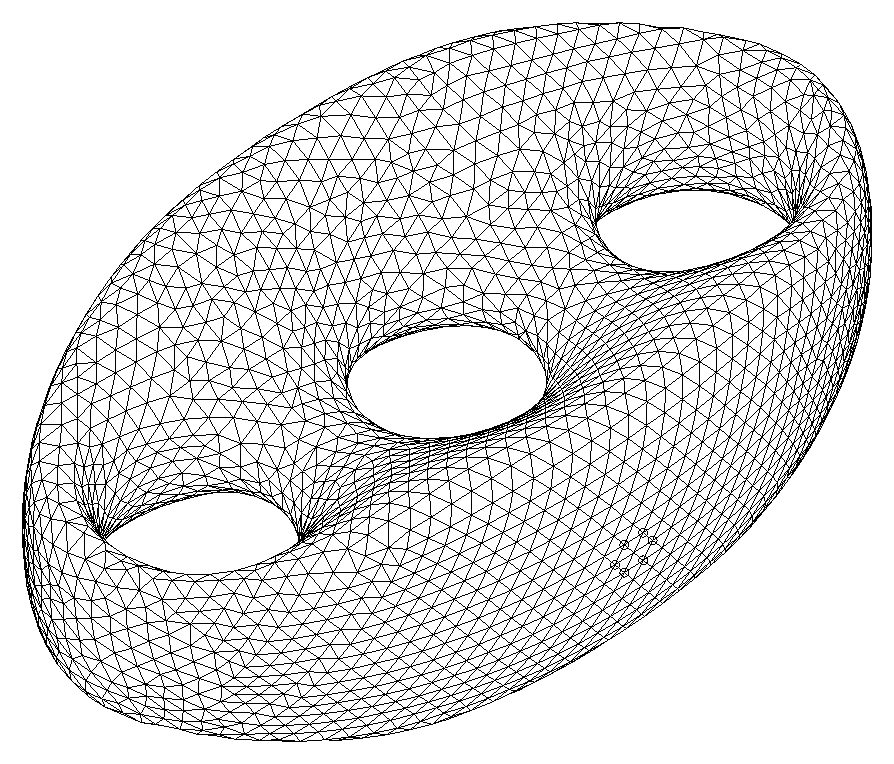
\includegraphics[width=200pt]{triangulated_genus3.pdf}
\caption{A 3-holes torus with triangulation, from Wikipedia. (\href{https://commons.wikimedia.org/wiki/File:Tri-brezel.svg}{By Ag2gaeh} - Own work, CC BY-SA 3.0.)}
\label{fig:genus3_wiki_triangulation}
\end{figure}

\subsection{Higher inductive combinatorial manifolds}

We will convert a simplicial complex \( M \) of dimension at most 2 to a higher inductive type, in two steps. 

\begin{mydef}
Define \( \combmfdt \) to be the type of \defemph{higher inductive constructors of combinatorial manifolds of dimension at most 2} and let \( \mathcal{H}:\combmfdsett\to\combmfdt \) be a map from a combinatorial manifold to such a HIT following this method:
\begin{enumerate}
\item vertices: a function \( \mathsf{v_0}:M_0\to \mathcal{H}(M) \) serving as the 0-dimensional constructors
\item edges: a function \( \mathsf{v_1} \) on 1-faces, sending \( \{a, b\}\mapsto \mathsf{v_0}(a)=\mathsf{v_0}(b) \)
\item 2-faces: a function \( \mathsf{v_2} \) on 2-faces, sending \( \{a, b, c\}\mapsto \refl_a = \mathsf{v_1}(\{a, b\})\cdot \mathsf{v_1}(\{b, c\})\cdot \mathsf{v_1}(\{a, c\})^{-1} \).
\end{enumerate}
\end{mydef}

We will assume there is a formal theory of such HITs, and that at least up to dimension 2 there are no obstructions to simply copying over the combinatorial data to the HIT constructors. For recent work on HITs see for example David Wärn's discussion of pushouts\cite{warn_pushouts}.

\begin{mydef}
Denote by \( \re:\combmfdt\to\Type \) the process of generating a type from the HIT data (which we refer to as \defemph{realization}). Note that \( \re(\mathcal{H}(M)) \) is not in general a set, and may not even be 2-truncated for an arbitrary 2-dimensional combinatorial manifold \( M:\combmfdsett \).
\end{mydef}

We're making the distinction between \( \mathcal{H} \) and \( \re \) because we will mostly study functions and phenomena on \( \mathcal{H}(M) \) for some simplicial complex \( M \).

\subsection{Polygons}\label{sec:polygons}

We will now start looking at some examples, first by defining a type that is important both for the domain and the codomain of mere circles: a square.

\begin{mydef}
The higher inductive type \( C_4 \) (where C stands for ``circle'').
\begin{align*}
C_4 &: \Type \\
c_1, c_2, c_3, c_4 &: C_4 \\
c_1c_2 &: c_1 = c_2 \\
c_2c_3 &: c_2 = c_3 \\
c_3c_4 &: c_3 = c_4 \\
c_4c_1 &: c_4 = c_1 \\
\end{align*}
\end{mydef}

\begin{figure}[htbp]
\centering
\begin{tikzpicture}[
node distance = 15mm and 15mm,
V/.style = {circle, fill, draw=black, inner sep=1pt, font=\footnotesize},
every edge quotes/.style = {auto, font=\footnotesize},
arrow/.style={->,semithick}
]
\begin{scope}[nodes=V]
  \node[label=above left:\( c_1 \)] (1) {};
  \node[label=above right:\( c_2 \)] (2) [right=of 1]  {};
  \node[label=below right:\( c_3 \)] (3) [below=of 2]  {};
  \node[label=below left:\( c_4 \)] (4) [below=of 1]  {};
\end{scope}
\draw[arrow]
        (1)  edge["\( c_1c_2 \)"] (2)
        (2)  edge["\( c_2c_3 \)"] (3)
        (3)  edge["\( c_3c_4 \)"] (4)
        (4)  edge["\( c_4c_1 \)"] (1);
\end{tikzpicture}

\caption{The HIT \( C_4 \).}
\end{figure}

The standard HoTT circle itself is a non-example of a combinatorial manifold since it lacks the second vertex of the edge:

\begin{mydef}
The higher inductive type \( \so \):
\begin{align*}
\so &:\Type \\
\mathsf{base}&:\so \\
\mathsf{loop}&:\mathsf{base}=\mathsf{base}
\end{align*}
\end{mydef}

Nonetheless, all polygons are equivalent to each other and to \( \so \).

\begin{mylemma}
\label{lem:c4equiv}
Define the function \( \ell:C_4\to\so \) by
\begin{align*}
\ell(c_i)&=\mathsf{base}, i=1, 2, 3, 4 \\
\ell(c_1c_2)&=\mathsf{loop} \\
\ell(c_2c_3)=\ell(c_3c_4)=\ell(c_4c_1)&=\refl_{\mathsf{base}}
\end{align*}
and define the function \( s_1:\so\to C_4 \) by \( s_1(\mathsf{base})=c_1 \) and \( s_1(\mathsf{loop})=c_1c_2\cdot c_2c_3\cdot c_3c_4\cdot c_4c_1 \). (The subscript on \( s_1 \) reminds us that we chose vertex \( c_1 \) to map \( \mathsf{base} \) to.) Then \( \ell \) and \( s_1 \) constitute an equivalence \( \mathsf{c4\_equiv}:\mathsf{is_equiv}(\ell,s_1) \).
\end{mylemma}
\begin{proof}
First we need to construct a term \( 4e:\pit{x:C_4}s_1(\ell(x))=x \) by induction on \( C_4 \), by defining terms
\begin{enumerate}
\item \( 4ei:s_1(\ell(c_i))=c_i \)
\item \( 4eij:\apd(c_ic_j)(4ei)=4ej \), i.e. \( 4eij: s_1(\ell(c_ic_j))^{-1}\cdot 4ei\cdot c_ic_j=4ej \).
\end{enumerate}
where in the second goal we used a result about \( \apd \) on transport (HoTT Book\cite{hottbook} Theorem 2.11.3). These goals are fulfilled by
\begin{itemize}
\item \( 4e1=\refl_{c_1} \)
\item \( 4e2={c_1c_2} \)
\item \( 4e3={c_1c_2\cdot c_2c_3} \)
\item \( 4e4={c_1c_2\cdot c_2c_3\cdot c_3c_4} \)
\item \( 4e12=(c_1c_2\cdot c_2c_3\cdot c_3c_4\cdot c_4c_1)^{-1}\cdot(-) \)
\item \( 4e23=\refl_{c_1c_2\cdot c_2c_3} \)
\item \( 4e34=\refl_{c_1c_2\cdot c_2c_3\cdot c_3c_4} \)
\item \( 4e41=4e12 \).
\end{itemize}
Next we need a term \( e4:\pit{y:S^1}\ell(s_1(y))=y \) by induction on \( S^1 \), by defining.
\begin{enumerate}
\item \( e4b:\ell(s_1(\mathsf{base}))=\mathsf{base} \)
\item \( e4l:\apd(\mathsf{loop})(e4b)=e4b \), i.e. \( e4l:\ell(s_1(\mathsf{loop}))^{-1}\cdot e4b\cdot e4b \).
\end{enumerate}
These goals are fulfilled by
\begin{itemize}
\item \( e4b=\refl_{\mathsf{base}} \)
\item \( e4l=\refl_{\mathsf{loop}} \).
\end{itemize}
\end{proof}
A different approach might be to prove that \( C_n\simeq C_{n-1} \) by removing just one vertex, and seeing that the argument generates equivalences between any polygon, or a polygon and \( S^1 \).

Recalling that terms of \( \EMzo \) are pairs: a type, and a mere equivalence with \( \so \), we have:

\begin{mycor}
We have \( (C_4,||\mathsf{c4\_equiv}||_{-1}):\EMzo. \)
\end{mycor}

Given some other square \( abcd \) and an equivalence with \( C_4 \), we get via univalence a path in \( \EMzo \). This includes automorphisms of \( C_4 \), for example \( R \). Furthermore there is a homotopy from \( R \) to the identity, which give a 2-path \( \refl_{C_4}=R \) in the universe.

Real-world triangulations of surfaces will often have links whose number of vertices varies across the surface. For example we can see hexagons and pentagons in Figure~\ref{fig:sphere_triangulation}. This presumably introduces only a minor practical inconvenience and doesn't materially affect the discussion to come.

\subsection{\texorpdfstring{The higher inductive type \( \oo \)}{The higher inductive type O}}

We will create our first combinatorial surface, a 2-sphere. We will adopt the convention that a subscript indicates the dimension of a subskeleton of a complex. For instance, we have \( \mathsf{base}:\so_0 \).

\begin{mydef}
The HIT \( \oo_0 \) is just 6 points, intended as the 0-skeleton of an octahedron, with vertices named after the colors on the faces of a famous Central European puzzle cube.
\[ w, y, b, r, g, o : \oo_0 \]
\end{mydef}

\begin{mydef}
The HIT \( \oo_1 \) is the 1-skeleton of an octahedron.
\begin{align*}
w, y, b, r, g, o &: \oo_1 & yg &: y=g \\
wb &: w=b & yo &: y=o \\
wr &: w=r & br &: b=r \\
wg &: w=g & rg &: r=g \\
wo &: w=o & go &: g=o \\
yb &: y=b & ob &: o=b \\
yr &: y=r
\end{align*}
\end{mydef}

\begin{mydef}
The HIT \( \oo \) is an octahedron:
\begin{align*}
w, y, b, r, g, o &: \oo \\
wb &: w=b & br &: b=r & wbr &: wb\cdot br\cdot wr^{-1} = \refl_w \\
wr &: w=r & rg &: r=g & wrg &: wr\cdot rg\cdot wg^{-1} = \refl_w \\
wg &: w=g & go &: g=o & wgo &: wg\cdot go\cdot wo^{-1} = \refl_w \\
wo &: w=o & ob &: o=b & wob &: wo\cdot ob\cdot wb^{-1} = \refl_w \\
yb &: y=b & & & yrb &: yr\cdot rb\cdot yb^{-1} = \refl_y \\
yr &: y=r & & & ygr &: yg\cdot gr\cdot yr^{-1} = \refl_y \\
yg &: y=g & & & yog &: yo\cdot og\cdot yg^{-1} = \refl_y \\
yo &: y=o & & & ybo &: yb\cdot bo\cdot yo^{-1} = \refl_y 
\end{align*}
\end{mydef}

\begin{figure}[htbp]
\centering
\begin{figure}[h]
\centering
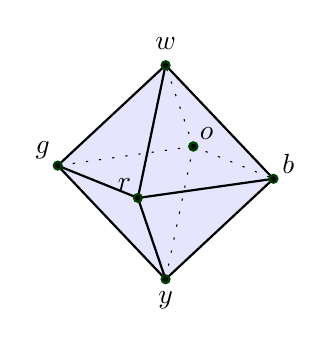
\begin{tikzpicture}%
  [x={(-0.860769cm, -0.121512cm)},
  y={(0.508996cm, -0.205391cm)},
  z={(-0.000053cm, 0.971107cm)},
  scale=1,
  back/.style={loosely dotted, thin},
  edge/.style={black, thick},
  facet/.style={fill=blue!95!black,fill opacity=0.1},
  vertex/.style={inner sep=1pt,circle,draw=green!25!black,fill=black,thick}]
\coordinate (-1, -1, 0) at (-1, -1, 0);
\coordinate (-1, 1, 0) at (-1, 1, 0);
\coordinate (0, 0, -1) at (0, 0, -1);
\coordinate (0, 0, 1) at (0, 0, 1);
\coordinate (1, -1, 0) at (1, -1, 0);
\coordinate (1, 1, 0) at (1, 1, 0);
%% Drawing edges in the back
%%
\draw[edge,back] (-1, -1, 0) -- (-1, 1, 0);
\draw[edge,back] (-1, -1, 0) -- (0, 0, -1.4);
\draw[edge,back] (-1, -1, 0) -- (0, 0, 1.4);
\draw[edge,back] (-1, -1, 0) -- (1, -1, 0);
%% Drawing vertices in the back
%%
\node[vertex] at (-1, -1, 0)     {};
%% Drawing the facets
%%
\fill[facet] (1, 1, 0) -- (0, 0, -1.4) -- (1, -1, 0) -- cycle {};
\fill[facet] (1, 1, 0) -- (0, 0, 1.4) -- (1, -1, 0) -- cycle {};
\fill[facet] (1, 1, 0) -- (-1, 1, 0) -- (0, 0, 1.4) -- cycle {};
\fill[facet] (1, 1, 0) -- (-1, 1, 0) -- (0, 0, -1.4) -- cycle {};
%% Drawing edges in the front
%%
\draw[edge] (-1, 1, 0) -- (0, 0, -1.4);
\draw[edge] (-1, 1, 0) -- (0, 0, 1.4);
\draw[edge] (-1, 1, 0) -- (1, 1, 0);
\draw[edge] (0, 0, -1.4) -- (1, -1, 0);
\draw[edge] (0, 0, -1.4) -- (1, 1, 0);
\draw[edge] (0, 0, 1.4) -- (1, -1, 0);
\draw[edge] (0, 0, 1.4) -- (1, 1, 0);
\draw[edge] (1, -1, 0) -- (1, 1, 0);
%% Drawing the vertices in the front
%%
\begin{scope}[nodes=vertex]
\node[label=above right:\( b \)] at (-1, 1, 0)     {};
\node[label=below:\( y \)] at (0, 0, -1.4)     {};
\node[label=above:\( w \)] at (0, 0, 1.4)     {};
\node[label=above left:\( g \)] at (1, -1, 0)     {};
\node[label=above left:\( r \)] at (1, 1, 0)     {};
\node[label=above right:\( o \)] at (-1, -1, 0)     {};
\end{scope}
\end{tikzpicture}
\caption{The HIT \( \oo \) which has 6 points, 12 1-paths, 8 2-paths.}
\end{figure}

\caption{The HIT \( \oo \) which has 6 points, 12 1-paths, 8 2-paths.}
\end{figure}

We have obvious maps \( \oo_0\xrightarrow[]{i_0} \oo_1\xrightarrow[]{i_1} \oo \) that include each skeleton into the next-higher-dimensional skeleton.

\subsection{Groupoid operations on higher inductive combinatorial manifolds}

Let \( M:\simcompt \) be a combinatorial 2-manifold and \( \mm\defeq\mathcal{H}(M):\combmfdt \) the corresponding higher inductive type. \( \mm \) has triangular 2-faces just as \( M \) does, except they are 2-paths in the HoTT sense. If two faces \( bca \) and \( bdc \) share the edge \( bc \) (see Figure~\ref{fig:concat}), then we can define an operation that combines the combinatorics of simplices with the higher groupoid operations generated by our HIT. 

Consider Figure~\ref{fig:concat} and the 2-paths \( bac: ba\cdot ac=bc \) and \( bdc: bd\cdot dc = bc \). The 2-path concatenation \( bac\cdot bdc^{-1} \) is a path in \( ba\cdot ac = bd\cdot dc \). And from there we see we have a 4-gon \( abdc:\refl_b=\refl_b \). In this way we can concatenate faces across common boundaries once we choose a common vertex (in this case \( b \)).

\begin{figure}[htbp]
\centering
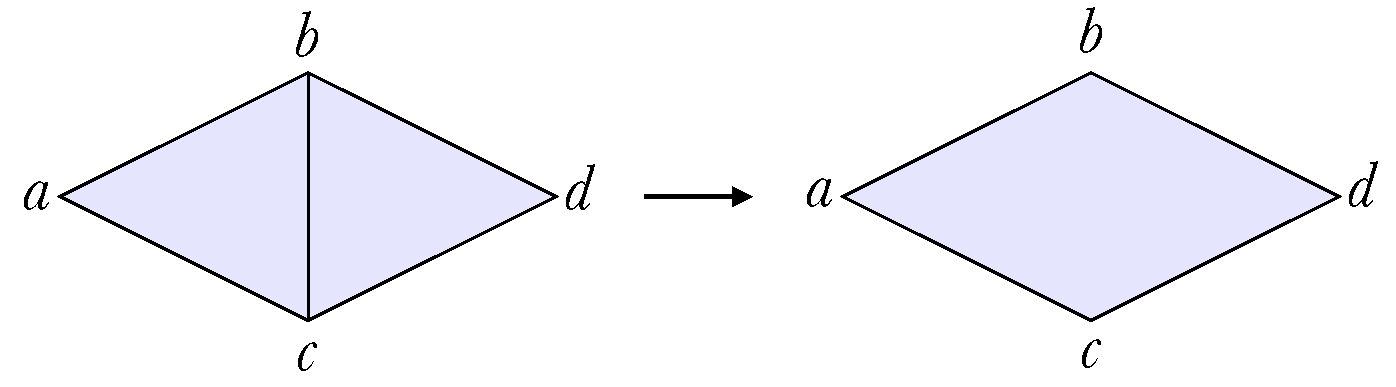
\includegraphics[width=250pt]{concat.pdf}
\caption{Concatenating the triangles \( bac \) and \( bdc \) gives the 4-gon \( abdc \).}
\label{fig:concat}
\end{figure}

We will have two use cases for this operation. The first is to consider the concatenation of \emph{all} the faces of \( \mm \), i.e. a term \( f_\mm:\refl_a=\refl_a \) corresponding to \( \mm \) itself. This will play the role of the ``fundamental homology class'' from classical topology, which is an object on which 2-forms can be evaluated to compute their value on the whole manifold. 

\begin{mydef}
\label{def:totalface}
If we have a combinatorial manifold \( \mm:\combmfdt \) (or a combinatorial manifold minus some isolated zeros \( \mm\defeq\mathbb{N}\setminus Z \)) and \( a:\mm_0 \) is a vertex, a \defemph{total face} of \( \mm \) is a term \( f_\mm:\refl_a=\refl_a \) given by any choice of ordering of the faces \( \{f_i\} \), a vertex \( v_i \) in each face, and terms \( a=v_i \) for each face.
\end{mydef}

Of course there are many choices in this definition of total face!

The second use case for concatenating faces is to create a HIT related to \( \mm \) but without some of the point constructors. Figure~\ref{fig:hex_concat} illustrates the equivalence.
\begin{figure}[htbp]
\centering
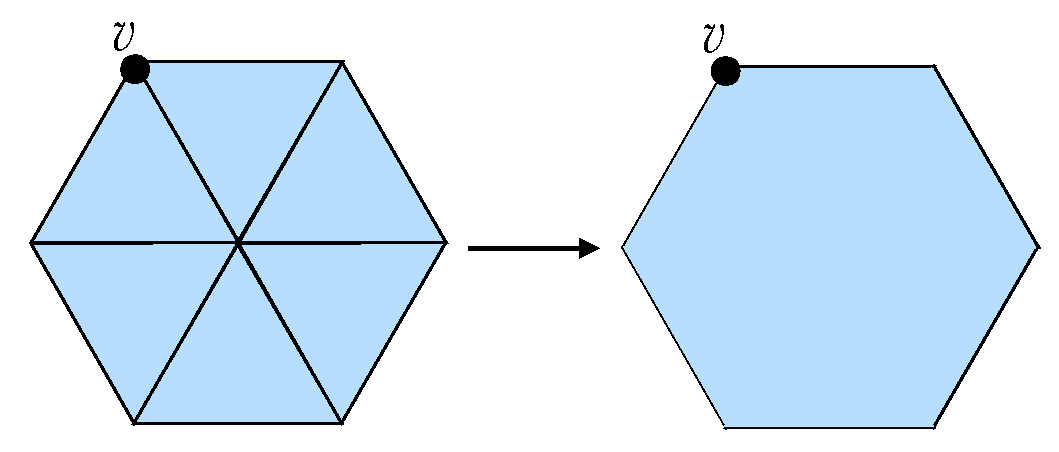
\includegraphics[width=200pt]{hex_concat.pdf}
\caption{Concatenating the six triangles in the approrpiate way produces a 2-path in \( \refl_v=\refl_v \) and removes the vertex at the center.}
\label{fig:hex_concat}
\end{figure}

\begin{mydef}
If \( \mm:\combmfdt \) is a combinatorial manifold and \( Z\subset \mm_0 \) is a set of vertices in \( \mm \) with members \( Z=\{z_0,\ldots,z_n\} \), then denote by \( \mm\setminus Z \) the type given by omitting the vertices in \( Z \) from the constructors in all dimensions where they appeared. Call the points of \( Z \) \defemph{isolated} if no two of them are neighbors, i.e. we have \( \pit{z:Z}\link(z)\cap Z=\emptyset \). In the isolated case \( \mm\setminus Z \) has boundary circles where each vertex was removed.
\end{mydef}

\begin{mydef}
\label{def:replacement}
If we have \( \mm\setminus Z \) for some isolated set of verticies \( Z \), then for each \( z:Z \) we can compose all the faces which contain \( z \), forming a new face (see Figure~\ref{fig:hex_concat}). In this way we produce a HIT called \( \mm_Z \), which is no longer combinatorial. We call \( \mm_Z \) the \defemph{replacement of \( \mm \) without \( Z \)}.
\end{mydef}

\begin{mylemma}
If \( Z \) are isolated points of \( \mm \) then we have \( \re(\mm)=_\Type\re(\mm_Z) \).
\end{mylemma}
\begin{proof}
We will prove that concatenating two faces of \( \mm \) as in Figure~\ref{fig:concat} produces an equivalent type. Let \( A \) be the constructor given on the left that includes the edge \( bc \), and \( B \) the constructor on the right. We will define functions on constructors. Let \( f:A\to B \) be
\begin{itemize}
\item \( f(a:A)=a:B, f(b)=b, f(c)=c, f(d)=d \)
\item \( f(ab)=ab, f(bd)=bd, f(dc)=dc, f(ca)=ca \)
\item \( f(bc)=bdc \)
\item \( f(abc)=abcd \)
\item \( f(bdc)=\refl_{bd\cdot dc} \)
\end{itemize} 
which ``squishes the right face onto its right >-shaped boundary.'' In the other direction let \( g:B\to A \) be the inclusion of all the constructors of dimension 1 and 2, and set \( g(abdc)=abc*bdc \), which denotes the concatenation operation across the shared edge.

We must provide a term \( gf:\pit{x:A}g(f(x))=x \) which requires supplying four paths, five pathovers, and two faceovers. The four paths are \( \refl_a \), \( \refl_b \), \( \refl_c \) and \( \refl_c \). Four of the pathovers are \( \refl_{ab} \), \( \refl_{bd} \), \( \refl_{dc} \), \( \refl_{ca} \). It remains to find terms 
\begin{enumerate}
\item \( \mathit{gfbc}:\apd(bc)(\refl_b)=\refl_c \)
\item \( \mathit{gfabc}:\apd(abc)(\refl_{ab}\cdot \mathit{gfbc}\cdot \refl_{ca})=\refl_{\refl_a} \), i.e. \( \mathit{gfabc}:g(f(abc))^{-1}\cdot  (\refl_{ab}\cdot \mathit{gfbc}\cdot \refl_{ca})\cdot abc = \refl_{\refl_a} \)
\item \( \mathit{gfbdc}:\apd(bdc)(\refl_{bd}\cdot \refl_{dc}\cdot \mathit{gfbc}^{-1})=\refl_{\refl_b} \), i.e. \( \mathit{gfbdc}:g(f(bdc))^{-1}\cdot (\refl_{bd}\cdot \refl_{dc}\cdot \mathit{gfbc}^{-1})\cdot bdc \)
\end{enumerate}
which are supplied by
\begin{enumerate}
\item \( cbd:cb\cdot bd\cdot dc=\refl_c \)
\item \( \refl_{\refl_{\refl_a}}\)
\item \( \refl_{\refl_{\refl_b}}\).
\end{enumerate}

We must also provide a term \( \mathit{fg}:\pit{x:B}f(g(x))=x \) which is \( \refl \) on all constructors.
\end{proof}
